%CONCEITOS---------------------------------------------------------------
\chapter{CONCEITOS}
\label{chap:conceitos}
O presente capítulo abordará os conceitos necessários para uma melhor compreensão dos artifícios utilizados para tratar o problema apresentado no Capítulo \ref{chap:introducao}, assim como uma
explanação sobre os extratores de características de imagens que serão utilizados e o estado da arte atual.

\section{ESPAÇOS MÉTRICOS} %TODO Ampliar
\label{sec:espmet}
Uma métrica em um conjunto $\mathbb{S}$ é uma função $d:\mathbb{S}$ $\times$ $\mathbb{S}$ $\rightarrow$ $\mathbb{R^{+}}$ que associa a cada par 
ordenado de elementos ($s_1$, $s_2$) um número real $d$($s_1$,$s_2$) chamado de distância de $s_1$ a $s_2$ \cite{Lima1977}.\par
Um espaço métrico $\mathbb{M}$ é um par <$\mathbb{S}$, $d$> onde $\mathbb{S}$ é um conjunto de elementos e $d$ é uma métrica
(ou função de distância). Esta distância $d$($s_1$,$s_2$) pode ser compreendido como uma medida de dissimilaridade entre dois elementos.
Quanto menor esta distância entre dois elementos, mais semelhantes eles são.
\begin{mydef}
 \label{def:espmet}
  Seja $\mathbb{S}$ um conjunto não-vazio de elementos e $d$($s_1$,$s_2$) uma métrica definida sobre $\mathbb{S}$ $\times$ $\mathbb{S}$.
   O par <$\mathbb{S}$, $d$> é chamado de espaço métrico desde que $d$ satisfaça as seguintes propriedades:\par
1. $d$($s_1$,$s_1$) = 0 (identidade);\par
2. Se $s_1$ $\neq$ $s_2$ ent\~ao $d$($s_1$,$s_2$) > 0 (n\~ao-negatividade);\par
3. $d$($s_1$,$s_2$) = $d$($s_2$,$s_1$) (simetria);\par
4. $d$($s_1$,$s_3$) $\leq$ $d$($s_1$,$s_2$) + $d$($s_2$,$s_3$) (desigualdade triangular)\\
onde $s_1$, $s_2$, $s_3$ $\in$ $\mathbb{S}$.
\end{mydef}
A importância prática do espaço métrico para este trabalho reside fortemente na quarta propriedade apresentada pela Definição \ref{def:espmet}. A desigualdade triangular é fundamentada na geometria euclidiana, 
onde a soma do comprimento de dois lados de um triângulo não pode ser superior ao comprimento do terceiro lado, como ilustra a figura \ref{fig:destri}.

\begin{figure}[H]
\centering
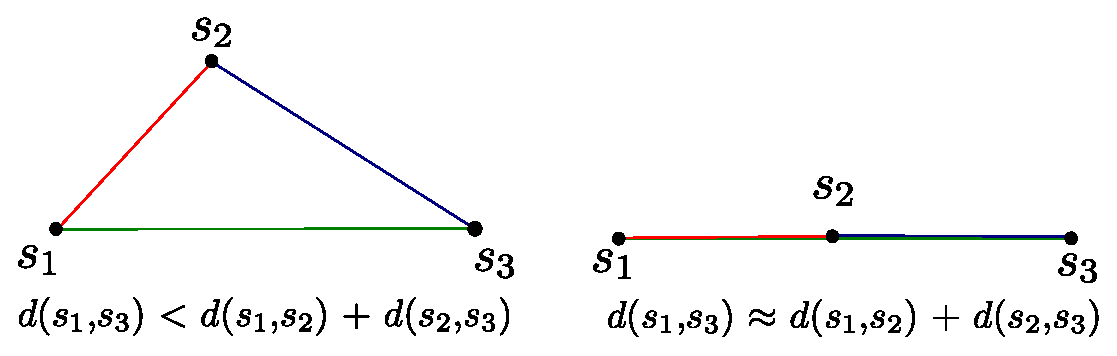
\includegraphics[width=.8\textwidth]{dados/figuras/desig_tri.eps}
\caption{Exemplo geométrico da desigualdade triangular}
\label{fig:destri}
\fonte{Autoria Própria}
\end{figure}

O emprego da desigualdade triangular neste trabalho será detalhado no capítulo \ref{chap:omni}.

\section{FUNÇÕES DE DISTÂNCIA}
\label{sec:funcdist}
Para verificar a similaridade entre dois elementos de um domínio, é utilizada uma função de distância. Esta função recebe como parâmetro um par
de elementos do conjunto e retorna o valor da dissimilaridade entre eles. Quanto mais próximo de zero, mais similares os elementos são.


%TODO Capítulo de conceitos! (estado da arte)(extratores de características)(espaços métricos)(funções de distância)(estruturas de indexação)(métricas)

%TODO % Para entender e ajustar os métodos de consultas por similaridade para diferentes tamanhos e tipos de conjuntos de dados, além de comparar diversos métodos, é importante uma análise teórica dos diferentes
% métodos de acesso e técnicas de estimativa do custo computacional \cite{POLA2010}. O cálculo do custo das operações realizadas será feito utilizando operações com B-trees, as quais o banco fornece suporte
% ao modelo de custo.

%TODO A solução abordada por esta proposta é a do uso de técnicas Omni, presentes no trabalho de \cite{Traina2001}. Um número calculado de elementos do conjunto de dados são selecionados como "focos", e utilizados para
% podar cálculos desnecessários de distâncias, fazendo uso da desigualdade triangular. Para quaisquer elementos $s_1$, $s_2$, $s_3$ $\in$ $\mathbb{S}$, sendo $\mathbb{S}$ um domínio de elementos
% e uma métrica $d : \mathbb{S} \times \mathbb{S} \rightarrow \mathbb{R^+}$, temos a desigualdade triangular:

% \begin{equation} \label{eq:destri}
% 		d(s_1,s_2) \leq d(s_1,s_3) + d(s_3,s_2)
% \end{equation}